\chapter[The HADES geometry]{The HADES geometry} \label{ch:geometry}

\section[Overview]{Overview}

The full HADES geometry needed to run a \textbf{simulation} is stored in Oracle:
\begin{itemize}
  \item ideal geometry
  \item different alignment versions for the simulation of beam times
  \item the information, which detector parts are present in a simulation project (or beam time).
\end{itemize}

The \textbf{geometry interface} (class HGeomInterface) allows
\begin{itemize}
   \item to read the media, geometry and hit definitions from Oracle and to create the geometry in
   \begin{itemize}
      \item \textbf{HGeant2} 
      \item the \textbf{ROOT geometry modeler} (class TGeoManager) for browsing, drawing, overlap checking and to 
        use eventually Virtual Monte Carlo (VMC) in the future
   \end{itemize}
   \item to create ASCII files and to read these files for initialization of HGeant2 and the ROOT TGeoManager
   \item to write the geometry and the parameters for hit definition into Oracle
   \item to generate geometry files taking into account the alignment of detectors
\end{itemize}
A \textbf{WebDB} interface provides access to the full geometry in \textbf{folder Geometry} (see~\ref{sec:oraGeometry}).

\begin{figure}[\htb]
  \centering
  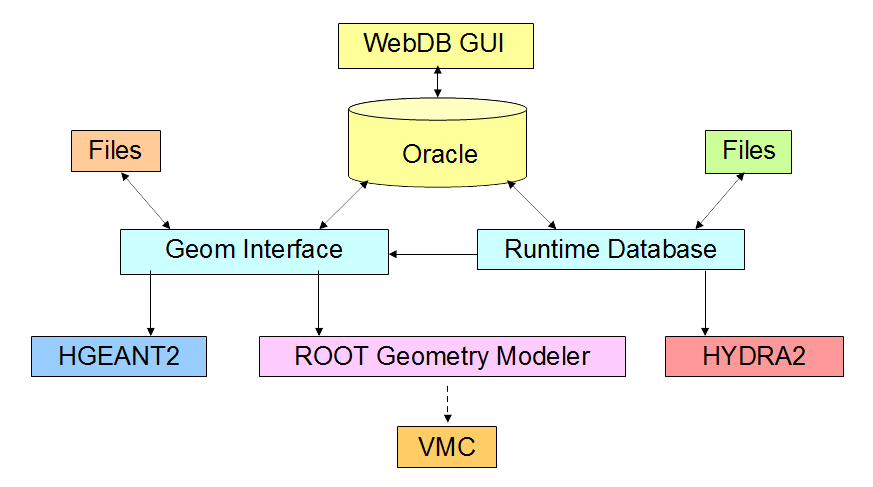
\includegraphics[scale=0.45]{hydra2_geom_overview}
  \caption[Geometry interfaces]{Geometry interfaces} \label{fig:geometryInterfaces}
\end{figure}

In the \textbf{analysis} only a small part of the geometry is needed for  digitization, tracking, and the event 
display. It is stored in parameter containers (see~Section:~\ref{sec:geomParameterContainers}) in the runtime database.


\section[Geometry classes]{Geometry classes} \label{sec:geometryClasses}

Fig.~\ref{fig:geomClasses} shows an overview of the geometry classes in Hydra2. The classes in the grey shaded area are 
implemented in hydra2/base/geometry. They are also used by the geometry parameter containers for the 
analysis (see~\ref{sec:geomParameterContainers}).\\

All other classes are only needed to create the geometry in HGeant2 or the ROOT TGeoManager (see \ref{sec:geomInterface}) 
and implemented in hydra2/simulation and hydra2/orasim.\\

\textbf{Hydra2 libraries needed for simulation:}
\begin{itemize}
  \setlength{\itemsep}{0pt}    
  \item libHydra
  \item libSimulation
  \item libOraSim (optional, requires the Oracle client installation)
\end{itemize}

\begin{figure}[\htb]
  \centering
  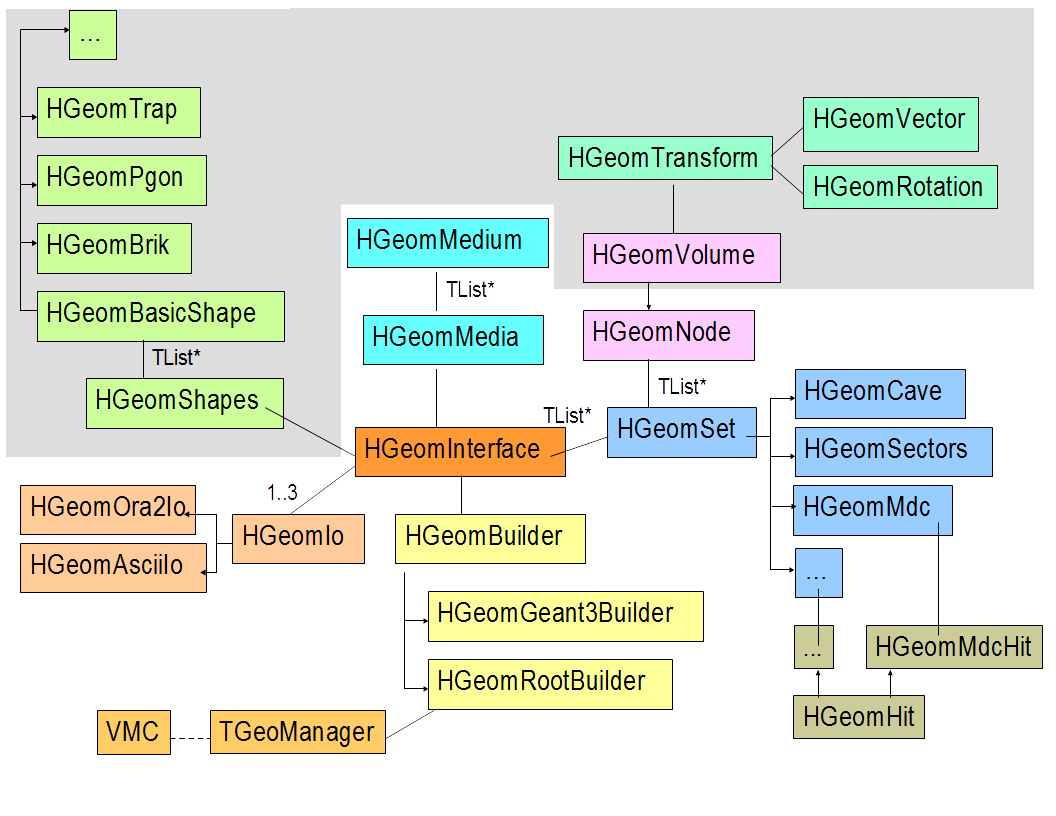
\includegraphics[scale=0.55]{hydra2_geom_classes}
  \caption[Geometry classes]{Geometry classes} \label{fig:geomClasses}
\end{figure}


\section[Detector sets]{Detector sets} \label{sec:geomDetectorSets}

All detector sets are derived from the base class \textbf{HGeomSet}, which implements most functionality.\\
The detectors typically only define some detector specific variables (detector name, number of keep-in volumes and number 
of modules) and simple functions, which return the name or the substring for keep-in volumes, modules and inner parts.\\

Detectors with sensitive volumes also have a class for the hit definition, derived from the base class \textbf{HGeomHit}.\\
The detector hit class only implements the function, which returns the IDTYP, the identifier of the hit set (eventually 
calculated from the name of the sensitive volume).

\subsection*{Cave}

\begin{tabular}{ll}
\emph{Keyword:}             & cave \\
\emph{Geom class:}          & HGeomCave \\
\emph{Parameter container:} & HSpecGeomPar 
\end{tabular}\\

It is a single volume with name CAVE and has no mother and therefore no transformation.\\
The origin (0.,0.,0.) of the local coordinate system of the cave is the same as the origin of the field map.\\
The ASCII file contains only this single volume. All daughters of the cave are defined in separate files.

\subsection*{Sectors}

\begin{tabular}{ll}
\emph{Keyword:}             & sectors \\
\emph{Geom class:}          & HGeomSectors \\
\emph{Parameter container:} & HSpecGeomPar 
\end{tabular}\\

The set consists of 6 volumes SEC1 ... SEC6 all with the same shape (PGON), medium and dimensions. Looking in beam 
direction the sectors are counted clockwise starting with the uppermost in positive y-direction.\\
All components of the translation vector describing the position of the sector coordinate system in the cave must be 0..

\subsection*{Rich}

\begin{tabular}{ll}
\emph{Keyword:}             & rich \\
\emph{Geom class:}          & HGeomRich \\
\emph{Parameter container:} & HRichGeometryPar 
\end{tabular}\\

The module (volume with name RICH sitting directly in the CAVE) contains a tree of volumes with names all starting with 'R'.\\
The volume RTAM is the mother volume for the target.\\

The analysis geometry container HRichGeometryPar is not derived from the base class HDetGeomPar and does not read any 
information from the standard geometry tables in Oracle. The RICH has its own tables (without version management), which 
are only for the ideal position (no alignment).

\subsection*{Target}

\begin{tabular}{ll}
\emph{Keyword:}             & target \\
\emph{Geom class:}          & HGeomTarget \\
\emph{Parameter container:} & HSpecGeomPar 
\end{tabular}\\

The target components (targets and support structures) sit in the RICH volume RTAM. To position the target components properly 
it is necessary to check the LAB-position of RTAM.\\
All target components have names starting with 'T'.\\
The targets must have the name TARG for a single target and TARGxx for a segmented target with identical segments, where xx 
is the number of the target. Several individual targets (different medium and/or size) must have names starting with 'TX'.\\
In an alignment geometry version the RICH is shifted, while the target volumes are at ideal z-position in the RICH.\\

The analysis interface reads only the target volumes from Oracle, not the support structure. To be independent from the RICH 
and to account for alignment, the transformation of all volumes is stored in the Lab-system.

\subsection*{MDC}

\begin{tabular}{ll}
\emph{Keyword:}             & mdc \\
\emph{Geom class:}          & HGeomMdc \\
\emph{Parameter container:} & HMdcGeomPar 
\end{tabular}\\

The MDC consists of 4 modules in each sector:\\
\begin{tabular}{ll}
plane 1 & DR1M1 ... DR1M6 \\
plane 2 & DR2M1 ... DR2M6 \\
plane 3 & DR3M1 ... DR3M6 \\
plane 4 & DR4M1 ... DR4M6
\end{tabular}\\
The dimensions of the modules in different sectors are the same, but can have different positions (alignment).\\
All sub-volumes in the MDC have names starting with "D1"..."D4".\\
The sensitive volumes (layers) must have 4-character names. The 4th character is the number of the layer (for example D1S4 
is the sensitive volume in layer 4 of plane 1).

\subsection*{TOF}

\begin{tabular}{ll}
\emph{Keyword:}             & tof \\
\emph{Geom class:}          & HGeomTof \\
\emph{Parameter container:} & HTofGeomPar 
\end{tabular}\\

The TOF wall consists of 8 TOF modules in each sector: \\
\begin{tabular}{rll}
  \textit{HGeant2 module index} & \textit{Volume names} & \textit{Analysis module index}\\
  15 & T15F1 ... T15F6 & 0 (outermost module)\\
  16 & T16F1 ... T16F6 & 1 \\
  17 & T17F1 ... T17F6 & 2 \\
  18 & T18F1 ... T18F6 & 3 \\
  19 & T19F1 ... T19F6 & 4 \\
  20 & T20F1 ... T20F6 & 5 \\
  21 & T21F1 ... T21F6 & 6 \\
  22 & T22F1 ... T22F6 & 7 \\
\end{tabular}\\
In HGeant the counting is done in positive y-direction and opposite in the analysis.
\footnote{The Tofino, a part of TOF in HGeant1 (module 22...26), was removed in Oracle for HGeant2, but the HGeant2 
FORTRAN code was not changed. A simulation with 22 TOF modules (without Tofino) was needed in the past by the kickplane 
algorithm to create new parameters.}\\
Each TOF module contains 8 identical sensitive cells (example T15S1 is the TOF rod closest to the beam line).

\subsection*{RPC}

\begin{tabular}{ll}
\emph{Keyword:}             & rpc \\
\emph{Geom class:}          & HGeomRpc \\
\emph{Parameter container:} & HRpcGeomPar 
\end{tabular}\\

The detector consists of one module in each sector: "ESKO1" ... "ESKO6". \\
All volumes have names starting with 'E', the sensitive cells with ``EG''. 

\subsection*{SHOWER}

\begin{tabular}{ll}
\emph{Keyword:}             & shower \\
\emph{Geom class:}          & HGeomShower \\
\emph{Parameter container:} & HShowerGeometry 
\end{tabular}\\

The Shower consists of a keep-in volume in each sector with names "SHK1" ... "SKH6".\\
Each keep-in volume contains 3 modules:\\
\begin{tabular}{ll}
module 1 & SH1M1 ... SH1M6 \\
module 2 & SH2M1 ... SH2M6 \\
module 3 & SH3M1 ... SH3M6
\end{tabular}\\
All  daughter volumes in the modules have names starting with "S1", "S2" and "S3".\\
Each module contains only one sensitive volume (for example S1AI in first module SH1M).
\footnote{In the analysis the cells are the wire planes S1SW...D3SW, daughters in the center of the sensitive volumes.}

\subsection*{Forward Wall}

\begin{tabular}{ll}
\emph{Keyword:}             & wall \\
\emph{Geom class:}          & HGeomWall \\
\emph{Parameter container:} & HWallGeomPar 
\end{tabular}\\

The Forward Wall consists of a single module with name "WALL" sitting directly in the CAVE.\\
All daughter volumes have names starting with 'W'. The name of the sensitive cells start with ``W00'' followed by a number 
1, 2, 3 for the different cell sizes and the copy numbers.

\subsection*{Start}

\begin{tabular}{ll}
\emph{Keyword:}             & start \\
\emph{Geom class:}          & HGeomStart \\
\emph{Parameter container:} & HStartGeomPar (only Start detector = module 0)
\end{tabular}\\

All volumes start with 'V'. The Start detector module has the name ``VSTA'' (mother volume ``RTAM`` in RICH), 
the Veto module, if present, the name ``VVET'' (mother volume ``RICH``). Some geometry versions contain additional volumes
for the delta-electron shielding.\\
For the pion beam times in 2014, the diamonds in the Start detector (VSTD1 \ldots VSTD9) were implemented as 
sensitive volumes with new code in HGeant2 and Hydra2. The Oracle storage and interfaces may change in the future, in 
case the layout would be different.

\subsection*{EMC (ECAL)}

\begin{tabular}{ll}
\emph{Keyword:}             & emc \\
\emph{Geom class:}          & HGeomEmc \\
\emph{Parameter container:} & HEmcGeomPar 
\end{tabular}\\

All daughter volumes start with'G'.\\
The EMC consists of one module in each sector: GMOM1 ... GMOM6, each containing 163 identical daughters. The name of the 
sensitive volume (Lead glass crystal) is 'GLEA'.\\
The parameters for the external tracking of the Cherenkov photons are stored in a parameter ROOT file (not in Oracle).

\subsection*{Coils}

\begin{tabular}{ll}
\emph{Keyword:}             & coils \\
\emph{Geom class:}          & HGeomCoils \\
\end{tabular}\\

The magnet coils consist of one module in each sector: CKIV1 ... CKIV6.\\
All volumes have names starting with 'C'.

\subsection*{Frames}

\begin{tabular}{ll}
\emph{Keyword:}             & frames \\
\emph{Geom class:}          & HGeomFrames \\
\end{tabular}\\

This set contains all support structures and beam pipes, which are not parts of a detector \footnote{The MDC frustum 
and the stiffener bars in MDC4 (do not fit into the keep-in volume) are defined here.}, as independent modules. All of 
them may have substructures.\\
All volumes have names starting with 'F'. A module can be positioned in the cave ( having a 4-character name "Fxxx") 
or in the sectors (having 5-character names "Fxxx1" ..."Fxxx6").

\subsection*{User defined modules}

\begin{tabular}{ll}
\emph{Keyword:}             & user \\
\emph{Geom class:}          & HGeomUser \\
\end{tabular}\\

This set allows to read and create up to 9 independent user defined modules (no common keep-in volume) with names
''U1KI1'' ... ''U1KI6'' up to  ''U9KI1'' ... ''U9KI6''. The 5th character is the number of the sector and is missing, 
if the volume sits directly in the CAVE.\\
All sub-volumes have names starting with "U1" ... "U9".


\section[HADES geometry formats]{HADES geometry formats} 

\subsection[Volume definition]{Volume definition} \label{sec:geomvolumeformat}

\paragraph{GEANT3 and ROOT:} ~\\
In \textbf{GEANT3 and ROOT} the volume size is specified with the minimum number of parameters needed and for most shapes 
\textbf{relative to the center} of a volume. A TUBE for example is described by three parameters: half length, inner and 
outer radius. The center of the volume is positioned relative to the center of the mother, described by x, y, z and a  
$3\times2$ rotation matrix.\\
In case the size of the volume changes asymmetrically (for example the tube gets longer at one end, but the daughters should 
keep their absolute positions), the center of the volume shifts. Not only the transformation of the volume relative to its 
mother must be changed, but also the transformations of its daughters to keep their position.\\
Furthermore, the orientation of the internal coordinate system is shape dependent, for example different for the trapezoid 
shapes TRAP and TRD1.\\
\textbf{All sizes, distances and positions are in cm.}

\paragraph{HADES:} ~\\
In the HADES geometry format, each volume has it own local coordinate system, which must \textbf{not} be positioned in the 
center of the volume. The transformation defined by a position vector and a $3\times3$ rotation matrix describes the transformation 
of the local coordinate system of the volume relative to the local coordinate system of its mother.\\
Some shapes are defined by a list of points (BOX, TRAP, TRD1, ...). This makes it easier to transfer the data from technical 
drawings into the file format, especially for trapezoids.\footnote{Originally it was intended to import the geometry data 
directly from 3D-CATIA drawings by marking the volume points in CATIA, export them as IGES files and store them in Oracle.}\\
The geometry interface calculates automatically the parameters and transformation needed to create the volume inside GEANT 
or ROOT.\\
\textbf{All sizes, distances and positions are in mm.}


\begin{figure}[\htb]
  \centering
  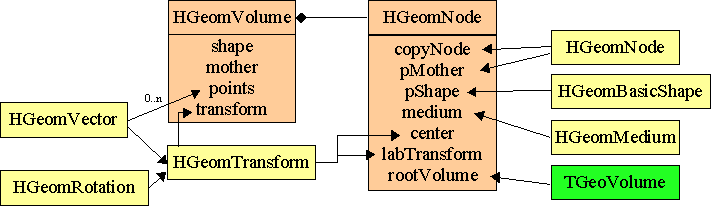
\includegraphics[scale=0.65]{hydra2_hgeomnode}
  \caption[The classes HGeomVolume and HGeomNode]{The classes HGeomVolume and HGeomNode} \label{fig:geomhgeomnode}
\end{figure}

A volume (except CAVE, which has no mother and therefore also no transformation) is defined by:
\begin{enumerate}
  \item name of the volume
  \item name of the mother volume
  \item GEANT shape of the volume
  \item name of the medium (= material)
  \item points or parameters from technical drawings (depend on the shape)
  \item position (x y z) of the coordinate system, in which the points are given, in the coordinate system of the mother
  \item $3\times3$ rotation matrix of the coordinate system listed row-wise as vector
\end{enumerate}

\paragraph{Names of volumes:} ~\\
All names start with a detector specific character (see \ref{sec:geomDetectorSets}~\nameref{sec:geomDetectorSets}). \\
Each volume has a name with at least 4 characters (upper case letters). Only the first 4 characters are used by GEANT (the 
name of the volume).\\
All volumes of which several copies exist (several nodes of the same volume) have names with 5 or more characters. These 
additional characters are always digits typically ranging from 1 to the maximum number of volumes with the same 
4-character GEANT name.\\
For example the outermost TOF (module number 22) contains 8 identical cells T22S1 ... T22S8. The volume T22S is created 
only once via GSVOLU(...) but positioned 8 times via GSPOS(...).\\
The names of the sensitive volumes must have a special structure defined for each detector.

\paragraph{Name of the mother:} ~\\
Each volume is positioned in a mother. The name of the mother has 4 characters (in upper case letters) plus eventually a 
number, if several copies of the mother exist. This number must be the number of the first node of the mother, typically 1.\\ 
(In GEANT only 4 characters are used, but the additional number is needed to find the mother in Oracle or in the file.)

\paragraph{GEANT Shape:} ~\\
Each volume has a shape (4 characters in upper case letters). Implemented in the program are the shapes \\
BOX~, PGON, PCON, TRAP, TRD1, TUBE, TUBS, CONE, CONS, SPHE, ELTU (see section~\ref{sec:geomShapes}).

\paragraph{Medium:} ~\\
Each volume is filled with a medium given by the name of the medium (see section~\ref{sec:geomMedia}). If not initialized 
from Oracle all media must be defined in a common media file.\\
The predefined media in GEANT are \textbf{not} used.

\paragraph{Points:} ~\\
Each volume has parameters describing the dimensions. The number of these parameters and their meaning depend on the 
shape of the volume. This is explained in section~\ref{sec:geomShapes}.

\paragraph{Coordinate system:} ~\\
Each volume has a local coordinate system in which the parameters are defined.\\
Its position and orientation relative to the coordinate system of the mother volume is described by a translation vector T 
and a 3x3 rotation matrix R according to the equation
\begin{verbatim}
     x=R*x'+T
\end{verbatim}
where x is the vector in the coordinate system of the mother and x' the vector in the coordinate system of the daughter.
The matrix R is listed row-wise as a vector with 9 components.\\
Each shape has its own intrinsic orientation, which is defined similar to the GEANT definition except for TRAP and TRD1 
(see~\ref{sec:geomShapes}).\\
As long as all volumes in a module are not rotated one may use the coordinate system of the module as the base coordinate 
system in which all points are given.\\

\textbf{Important: } The rotation matrix must be specified with a precision of at least $10^{-6}$. Otherwise one may get a 
lot of warnings from GEANT that the coordinate system is not orthogonal. The ROOT overlap checker would also detect them 
as overlaps or extrusions.\\
Furthermore it may cause rounding problems when storing the geometry in Oracle, because here the transformations of all 
inner volumes are stored relative to the module coordinate system even for multiple rotations.\\ 

Volumes of which several copies exist may use a shortened input structure in the ASCII file:\\
For the first volume all information above must be defined. For the other copies specified later in the file one must only 
specify
\begin{itemize}
  \setlength{\itemsep}{0pt}    
  \item name of the volume
  \item name of the mother
  \item translation vector of the coordinate system
  \item rotation matrix of the coordinate system
\end{itemize}


\subsection[Volume shapes]{Volume shapes} \label{sec:geomShapes}

Each shape is defined by a variable number of 'points' (one in each line of the input file), each having 1-3 components. 
Apart from the shapes with 8 corners (BOX~, TRAP, TRD1) the parameter are partially similar to the ones in GEANT.
Each shape has an intrinsic coordinate system. They have the same orientation as in GEANT except for TRAP and TRD1.

\begin{figure}[\htb]
  \centering
  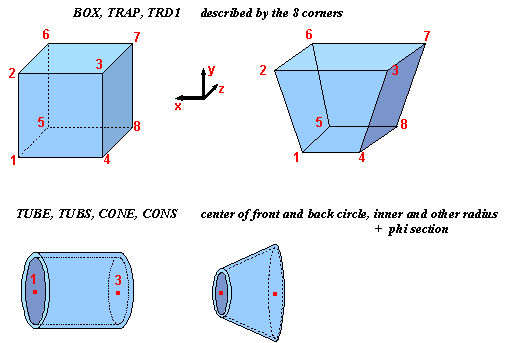
\includegraphics[scale=0.85]{hydra2_geom_shapes}
  \caption[Some volume shapes]{Some volume shapes} \label{fig:geomtryShapes}
\end{figure}

\paragraph{BOX} (class HGeomBrik)\\
It has 8 corners described by the x, y, z coordinates.\\
For example the master volume CAVE is implemented as a large BOX.

\paragraph{TRAP} (class HGeomTrap)\\
The coplanar front and back planes are trapezoids with centers not necessarily on a line parallel to the z-axis. Typical 
examples are the MDC modules with back planes larger than the front planes.\\
A TRAP has 8 corners described by the x, y, z coordinates. The corners are counted clockwise starting at the lower left 
corner of the front plane.\\
The intrinsic coordinate system of a TRAP is different from the one in GEANT. The y-axis points from the smaller side in 
x-direction to the larger one. A TRAP not rotated in a BOX has the same intrinsic coordinate system as the BOX. In GEANT 
the y- and x-axis point in the opposite directions.

\paragraph{TRD1} (class HGeomTrd1)\\
The coplanar front and back planes are trapezoids of the same size and with centers on a line parallel to the z-axis. 
Examples are the MDC wire planes.\\
The shape has 8 corners described by the x, y, z coordinates. In HADES the intrinsic coordinate system of a TRD1 is the 
same as for a TRAP, different from the definition in GEANT.

\paragraph{PGON} (class HGeomPgon)\\
The polygon has a variable number of points with 1-3 components:\\
\begin{tabular}{|l|l|}
  \hline
  point 0                    & NZ number of planes perpendicular to the z-axis where the section is given\\
  \hline
  \multirow{3}{*}{point 1}   & azimuthal angle PHI1 at which the volume begins\\
                             & opening angle DPHI of the volume\\
                             & number NPDV of sides of the cross section between the phi limits\\
  \hline
  \multirow{3}{*}{point 2ff} & z coordinate Z of the section\\
                             & inner radius RMIN at position z\\ 
                             & outer radius RMAX at position z\\
  \hline
\end{tabular}\\[1.5px]
The sectors SEC1...SEC6 are implemented as PGON.

\paragraph{PCON} (class HGeomPcon)\\
The polycon has a variable number of points with 1-3 components:\\
\begin{tabular}{|l|l|}
  \hline
   point 0                   & NZ number of planes perpendicular to the z-axis where the section is given\\
  \hline
  \multirow{2}{*}{point 1}   & azimuthal angle PHI1 at which the volume begins\\ 
                             & opening angle DPHI of the volume\\
  \hline
  \multirow{3}{*}{point 2ff} & z coordinate Z of the section\\
                             & inner radius RMIN at position z\\
                             & outer radius RMAX at position z\\
  \hline
\end{tabular}\\[1.5px]
The RICH volume RMET filled with Methan is implemented as PCON.

\newpage
\paragraph{SPHE} (class HGeomSphe)\\
Is is a spherical shell segment described by 3 points with 2 components:\\
\begin{tabular}{|l|l|}
  \hline
  \multirow{2}{*}{point 0} & inner radius RMIN of the shell\\ 
                           & outer radius RMAX of the shell\\
  \hline
  \multirow{2}{*}{point 1} & starting polar angle THE1 of the shell\\ 
                           & ending polar angle THE2 of the shell\\
  \hline
  \multirow{2}{*}{point 2} & starting azimuthal angle PHI1 of the shell\\ 
                           & ending azimuthal angle PHI2 of the shell\\
  \hline
\end{tabular}\\[1.5px]
The RICH mirror RMIR is implemented as SPHE.

\paragraph{TUBE} (class HGeomTube)\\
This shape has 3 points with 2-3 components:\\
\begin{tabular}{|l|l|}
  \hline
  point 0                  & x, y, z coordinate of the center of the circle at the beginning of the TUBE\\
  \hline
  \multirow{2}{*}{point 1} & inner radius RMIN\\
                           & outer radius RMAX\\
  \hline
  point 2                  & x, y, z coordinate of the center of the circle at the end of the TUBE\\
  \hline
\end{tabular}\\[1.5px]
Typical examples are the solid targets (with RMIN = 0).

\paragraph{TUBS} (class HGeomTubs)\\
A TUBS is a segment of a TUBE. It has 4 points with 2-3 components:\\
\begin{tabular}{|l|l|}
  \hline
  point 0                  & x, y, z coordinate of the center of the circle at the beginning of the TUBS\\
  \hline
  \multirow{2}{*}{point 1} & inner radius RMIN\\
                           & outer radius RMAX\\
  \hline
  point 2                  & x, y, z coordinate of the center of the circle at the end of the TUBS\\
  \hline
  \multirow{2}{*}{point 3} & starting angle PHI1 of the segment\\
                           & ending angle PHI2 of the segment\\
   \hline
\end{tabular}\\[1.5px]
Examples are the 60 degree segments of the Carbon beam pipe FOUC1...FOUC6, one in each sector.

\paragraph{CONE} (class HGeomCone)\\
This conical tube has 4 points with 2-3 components:\\
\begin{tabular}{|l|l|}
  \hline
  point 0                  & x, y, z coordinate of the center of the circle at the beginning of the CONE\\
  \hline
  \multirow{2}{*}{point 1} & inner radius RMN1 at the beginning of the CONE\\
                           & outer radius RMX1 at the beginning of the CONE\\
  \hline
  point 2                  & x, y, z coordinate of the center of the circle at the end of the CONE\\
  \hline
  \multirow{2}{*}{point 3} & inner radius RMN2\ at the end of the CONE\\
                           & outer radius RMX2 at the end of the CONE\\
  \hline
\end{tabular}\\[1.5px]
An example is the volume TARG (filled with liquid Hydrogen) of the LH2 target.

\paragraph{CONS} (class HGeomCons)\\
A CONS is a segment of a CONE. It has 5 points with 2-3 components:\\
\begin{tabular}{|l|l|}
  \hline
  point 0                  & x, y, z coordinate of the center of the circle at the beginning of the CONS\\
  \hline
  \multirow{2}{*}{point 1} & inner radius RMN1\ at the beginning of the CONS\\
                           & outer radius RMX1 at the beginning of the CONS\\
  \hline
  point 2                  & x, y, z coordinate of the center of the circle at the end of the CONS\\
  \hline
  \multirow{2}{*}{point 3} & inner radius RMN2\ at the end of the CONS\\
                           & outer radius RMX2 at the end of the CONS\\
  \hline
  \multirow{2}{*}{point 4} & starting angle PHI1 of the segment\\
                           & ending angle PHI2 of the segment\\
   \hline
\end{tabular}

\paragraph{ELTU} (class HGeomEltu)\\
This shape has 3 points with 2-3 components:\\
\begin{tabular}{|l|l|}
  \hline
  point 0                  & x, y, z coordinate of the center of the ellipsoid at the beginning of the ELTU\\
  \hline
  \multirow{2}{*}{point 1} & semi-axis P1 along x\\
                           & semi-axis P2 along y\\
  \hline
  point 2                  & x, y, z coordinate of the center of the ellipsoid at the end of the ELTU\\
  \hline
\end{tabular}

\paragraph{Important:} A TUBE, TUBS, CONE, ELTU cannot be rotated by different x- and y-values of the starting and ending 
circles or ellipsoids. They have to be identical. A rotation can only be defined by a rotation matrix.


\subsection[Material and media definition in HGeant2]{Material and media definition in HGeant2}\label{sec:geomMedia}
\begin{itemize}
 \item Each medium is characterized by a name\\
       HADES naming convention: capital letters, ending with \textbf{\$}.
 \item The names of the materials and the media in GEANT are identical.
 \item For each medium all parameters needed by the GEANT routines GSMATE, GSMIXT, GSTMED and GSCKOV are defined.
 \item The predefined materials in GEANT are not used.
\end{itemize}

The following parameters are needed:\\
\begin{tabular}{|l|l|}
  \hline
  \cellcolor{lightgray} \textit{Parameter} & \cellcolor{lightgray} \textit{Description}\\
  \hline
  \multirow{4}{*}{int ncomp} & number of components in the material\\
                             & ncomp = 1 for a basic material\\
                             & \textgreater 1 mixture, WMAT contains the proportion by weights\\
                             & \textless 1 mixture, WMAT contains the proportion by number of atoms\\
  \hline
  float aw[ncomp]            & atomic weights A for the components\\
  \hline
  float an[ncomp]            & atomic numbers Z for the components\\
  \hline
  float dens                 & density DENS in g cm(**-3)\\
  \hline
  float radleng              & radiation length RADL (only for a basic material)\\
  \hline
  loat wm[ncomp]             & weights WMAT of each component in a mixture (only for a mixture)\\
  \hline
  int sensflag               & sensitivity flag ISVOL (1 for sensitive media, 0 for insensitive ones)\\
  \hline
  int fldflag                & field flag IFIELD\\
  \hline
  float fld                  & maximum field value FIELDM in kilogauss\\
  \hline
  float epsil                & boundary crossing precision EPSIL\\
  \hline
  int npckov                 & number of values used to define the optical properties of the medium.\\
  \hline
\end{tabular}\\[1.5ex]
Comments can only be placed \textbf{before} a medium definition in separate lines all starting with \verb+//+.\\

Examples:
\begin{lstlisting}
GOLDTARGET$
1  196.967  79  19.3  0.33508
0  1  15  0.001
0

// sensitive medium with 2 components specified by number of atoms in the mixture
SCINTILLATOR$
-2  12.011  1.008  6  1  1.03  9  10  
1  0  15  0.001
0
\end{lstlisting}

The variable \textbf{npckov} is 0 for all optically inactive media except some special media used in the RICH and 
in the ECAL to track the Cerenkov photons.\\
These media have additional parameter arrays:\\
\begin{tabular}{|l|l|}
  \hline
  float ppckov[npckov] & photon momentum in eV\\
  \hline
  float absco[npckov]  & absorption length in case of dielectric and of absorption probabilities in case of a metal\\
  \hline
  float effic[npckov]  & detection efficiency\\
  \hline
  float rindex[npckov] & refraction index for a dielectric, rindex[0]=0 for a metal\\
  \hline
\end{tabular}\vspace*{2ex}

The following parameters used in the GEANT tracking routines are normally not read. The default values are -1 and the real 
values are automatically calculated by GEANT.\\
\begin{tabular}{|l|l|}
  \hline
  float madfld & maximum angular deviation TMAXFD due to the field\\
  \hline
  float maxstep & maximum step permitted STEMAX\\
  \hline
  float maxde & maximum fractional energy loss DEEMAX\\
  \hline
  float minstep & minimum value for step STMIN\\
  \hline
\end{tabular}\vspace*{1.5ex}

To set the values explicitly one must add the following line in the medium file:
\begin{lstlisting}
AUTONULL
\end{lstlisting}
After this keyword each medium must specify these 4 parameters in one additional line.


\subsection[Hit definition in HGeant2]{Hit definition in HGeant2}

The file names for the hit definition must have the suffix \textbf{.hit} and contain the detector specific keyword ``rich``, 
''mdc'', ...(see section \ref{sec:geomDetectorSets}~\nameref{sec:geomDetectorSets}).\\
The files must contain the following parameters, needed for the GEANT routines GSDET and GSDETH:\\
\begin{tabular}{|l||l|l|}
  \hline
  \cellcolor{lightgray} \textit{Line} & \cellcolor{lightgray} \textit{Variable} & \cellcolor{lightgray} \textit{Description}\\
  \hline
  1 & string CHSET & the name of the hit set\\
  \hline
  2 & int NH & the number of hit components (maximum 30)\\
  \hline
  3 & string array CHNAMH & NH names of the hit components\\
  \hline
  4 & int array NBITSH    & NH numbers of bits in which to pack the components of the hits\\
  \hline
  5 & float array ORIG    & NH numbers of offsets applied before packing the hit values\\
  \hline
  6 & float array FACT    & NH numbers of scale factors applied before packing the hit values\\
  \hline
\end{tabular}\\

Comments can only be placed \textbf{before} a detector hit definition as separate lines all starting with \verb+//+.\\

Example:
\begin{lstlisting}
// Forward Wall hit definition
WLSC
11
   X       Y       Z       TOF     PART    ITRA    ELOS    IDET    PMOM    INWV    TLEN 
     30      30      30      30       8      14      30      12      30       4      30 
 340.00  340.00  340.00    0.00    0.00    0.00    0.00    0.00    0.00    0.00    0.00 
1.0e+04 1.0e+04 1.0e+04 1.0e+12 1.0e+00 1.0e+00 1.0e+07 1.0e+00 1.0e+07 1.0e+00 1.0e+04 
\end{lstlisting}


\section[Geometry interface for HGeant2 and ROOT]{Geometry interface for HGeant2 and ROOT} \label{sec:geomInterface}

\subsection[Configuration file geaini.dat]{Configuration file geaini.dat} \label{sec:geomGeaini}

The configuration file for HGeant2 consists of three parts:
\begin{enumerate}
 \setlength{\itemsep}{0pt}
 \item The list of GEANT key words and parameters ended with \verb+END+
 \item The geometry configuration and eventually a parameter ROOT file
 \item The field map, optional list of event input files, configuration of the ROOT output tree and output file name
\end{enumerate}
Part 1 is read only relevant for a simulation and read by the HGeant2 subroutine \verb+hgeakey.F+.\\
Part 2 and 3 are read in HGeant2 by the c++ function \verb+HGeantInput::readFileNames()+ and stored in various data members depending 
on special keywords or name/file extensions.\\

Described here is only the initialization part of the geometry.\\
In HGeant2 the function \verb+hgeomcreatesetup.cc+ (called from \verb+ugeom.F+) instantiates the geometry interface \verb+HGeomInterface+, 
configures it (sets the builder \verb+HGeomGeant3Builder+, file or Oracle input, parameter file), sets the run id and reads and 
creates the geometry.\\
In a pure Hydra2 application, for example the creation of geometry files from Oracle (see~\ref{sec:geomCreateGeoFiles}), 
part 2 of the configuration file is read by the geometry interface. Part 1 and 3, if existing, are ignored.\\  

Example: Configuration file for an APR12SIM simulation:
\begin{lstlisting}
!
! GEANT key words
!
PMCF 1
AUTO 1
KINE 0
FMAP 2
FPOL 0.7215
MXST 25000
JVER 2 2 0
BEAM 1. 1. 1230. 0. 0. 0.
SECO 3 1
CKOV 1
LOSS 1
DRAY 1
SWIT 0 0 0 0 0 1 0
TRIG TRIGGER_NUM
ETA  37.30 30.20 21.00 4.75 6.0 7.1e-2
TIME 0 1000000 1000000
SPLIT 1800000000
FILE 1
END            ! End of gffread
//
// ******************************************************************
//
// ---- geometry initialized from Oracle  ---------------------------
SimulRefRunDb:   apr12sim_mediumfieldalign_auau
HistoryDateDb:   now
//
// ******************************************************************
//
// ---- field map  --------------------------------------------------
/cvmfs/hades.gsi.de/param/field/fldrpz_unf.map
//
// ---- branches in the ROOT output tree  ---------------------------
kine.tup
rich.tup
mdc.tup
tof.tup
shower.tup
wall.tup
rpc.tup
//
// ---- input file(s)  ----------------------------------------------
/misc/kempter/projects/AuAu/run_urqmd/out/Au15Au_urqmd_bmax4_1000evts.evt
//
// ----  output file  -----------------------------------------------
test.root
\end{lstlisting}

\subsection{Keywords and file extensions} \label{sec:geomGeainiKeywords}

Special \textbf{keywords} (specified as "keyword" + ": " + "value") and \textbf{file extensions} are used to read and 
create the geometry.
\begin{itemize}
 \item \textbf{DbSupport:}\\
   This keyword accepts two values:
   \begin{itemize}
     \setlength{\itemsep}{0pt}
      \item \textbf{ON} (default)\\
      This creates the Oracle interface class HGeomOra2Io.    
      \item \textbf{OFF}
      In this case the geometry must be fully initialized from .geo and .hit files. This is the \textbf{standard value 
      when running a simulation on the batch farm}.    
    \end{itemize}
 \item \textbf{SimulRefRunDb:}\\
   This is the keyword to read the \textbf{full} geometry including the hit definition from Oracle.\\
   The value is the name of a simulation reference run. This defines the detector setup and the geometry version of each 
   detector part. The corresponding run id is set in the event header of the ROOT output file.
   \begin{lstlisting}
SimulRefRunDb:   apr12sim_mediumfieldalign_auau
   \end{lstlisting}
 \item \textbf{HistoryDateDb:}\\
   This is the keyword to set the history date of the geometry in Oracle.\\
   As in the analysis by default the geometry of the last parameter release for the simulation project is read from Oracle or 
   `` now'' if no release exists.
   \begin{lstlisting}
HistoryDateDb:   now
//HistoryDateDb:   01-NOV-2013 00:00:00
   \end{lstlisting}
 \item \textbf{ParameterFile:}\\
   With this keyword one may specify a parameter ROOT file for example needed to create the MDC geometry with wires or to read the 
   histograms for the external tracking of Cerenkov photons in the ECAL modules and the lookup table for the photomultipliers.
 \item \textbf{SimulRefRunId:} (HGeant2 only)\\
   With DbSupport OFF the run id is by default 0. In the analysis one needs to set the reference run id for initialization.\\
   As an alternative one can set the run id here and this way add it in the event header of the output file.
 \item \textbf{DebugFile:} (HGeant2 only)\\
   For debugging of a new geometry it might be helpful to get the parameters calculated by the program and used to call the
   GEANT FORTRAN routines. The file extension must be ``.txt''.
 \item \textbf{.geo}\\
   This is the file extension of the geometry or media ASCII files. For a detector with sensitive volumes also the corresponding 
   .hit file must be defined.
 \item \textbf{.hit}\\
   This is the file extension of an ASCII file containing the hit definition of a detector with sensitive volumes.
 \item \textbf{\_gdb}\\
   It is possible to mix input from Oracle and input from file. The part of the HADES detector read from Oracle is 
   specified by
   \begin{lstlisting}
     "keyword for the detector part" + "_gdb"
   \end{lstlisting}
   \textbf{All media must be read from file.}\\
   In the example below the media and the target are read from file, the CAVE and the RICH from Oracle. All other parts are 
   missing and therefore not created.\footnote{By reading only the media from file and some other parts from Oracle 
   it is possible to create only a subset of the HADES detector.}
   \begin{lstlisting}
SimulRefRunDb:   apr12sim_mediumfieldalign_auau
HistoryDateDb:   now
//
/misc/ilse/svn/hydra2/macros/Geom/pion/media_new.geo
cave_gdb
rich_gdb
/misc/ilse/svn/hydra2/macros/Geom/pion/target_new.geo
   \end{lstlisting}
 \item \textbf{.setup}\\
   Independent if one reads from Oracle or from files, always the full setup of the detectors is read and would be created.\\
   \textbf{In Hydra2 the default setup for the MDC are 24 modules and for the TOF the 8 outer modules.}\\
   To create only a subset of detectors one must specify a file with extension \textbf{.setup} in the configuration file.\\
   Below is an example how to define subsets:
   \begin{lstlisting}
// ----------------------------------------------------------------------
// Line 1 containes the detector name (lower-case) in [] brackets.
// Line 1 - 6 specifiy the setup in each sector with 1 = "in setup",
//                                                   0 = "not in setup".
// ----------------------------------------------------------------------
// NOV02 MDC setup
[mdc]
SEC1 1 1 1 1
SEC2 1 1 0 0
SEC3 1 1 1 0
SEC4 1 1 1 1
SEC5 1 1 0 0
SEC6 1 1 1 0
   \end{lstlisting}

\end{itemize}


\subsection[Production of geometry ASCII files for HGeant2]{Production of geometry ASCII files for HGeant2} 
\label{sec:geomCreateGeoFiles}

The interface allows to store the geometry read from Oracle in ASCII files. Then these file may be used for 
initialization for example on the batch farm.

\paragraph{1. Step: Configuration file} ~\\
The file must contain the name of the simulation reference run and eventually a history date, but no .geo or .hit files.\\
Example: ora2files.dat
\begin{lstlisting}
SimulRefRunDb:   apr12sim_mediumfieldalign_auau
HistoryDateDb:   now
\end{lstlisting}

\paragraph{2. Step: ROOT macro ora2files.C} ~\\
One must only specify the configuration file and the output directory. 
\begin{lstlisting}
{
  // configuration file
  TString configFile = "ora2files.dat";

  // output directory (must exist)
  TString outputDir = "./geom12001";

  // ******************************************************

  HGeomInterface* interface=new HGeomInterface;

  HGeomOra2Io* oraInput=new HGeomOra2Io;
  oraInput->open();
  interface->setOracleInput(oraInput);

  Bool_t rc=interface->readGeomConfig(configFile.Data());

  HGeomAsciiIo* output=new HGeomAsciiIo;
  output->setDirectory(outputDir.Data());
  interface->setOutput(output);

  Bool_t rc=interface->readAll();
  if (rc) {
    interface->writeAll();
    // HGeomSet* set=interface->findSet("target");
    // if (set) interface->writeSet(set);
    // interface->writeMedia();
  }
  delete interface;
}
\end{lstlisting}

It generates separate files for the media and all detector parts with file names
\begin{lstlisting}
    "keyword for the detector part" + "actual date and time" + ".geo"
\end{lstlisting}
and for detectors with sensitive volumes also the hit files with extension ".hit".\\

The commented lines show an example how to write only a single .geo file.


\subsection[Initialization from ASCII Files]{Initialization from ASCII Files}
With all .geo and .hit files created from Oracle one can switch OFF the Oracle support and replace the geometry part in 
the configuation file:
\begin{lstlisting}
//
// SimulRefRunDb:   apr12sim_mediumfieldalign_auau
// HistoryDateDb:   now
//
DbSupport:     OFF
SimulRefRunId: 12001
//
geom12001/media_230615155440.geo
geom12001/cave_230615155440.geo
geom12001/rich_230615155440.geo
geom12001/target_230615155440.geo
geom12001/sect_230615155440.geo
geom12001/mdc_230615155440.geo
geom12001/coils_230615155440.geo
geom12001/tof_230615155440.geo
geom12001/shower_230615155440.geo
geom12001/frames_230615155440.geo
geom12001/start_230615155440.geo
geom12001/wall_230615155440.geo
geom12001/rpc_230615155440.geo
//
geom12001/rich_230615155440.hit
geom12001/mdc_230615155440.hit
geom12001/tof_230615155440.hit
geom12001/shower_230615155440.hit
geom12001/start_230615155440.hit
geom12001/wall_230615155440.hit
geom12001/rpc_230615155440.hit
\end{lstlisting}

If a file is missing, the corresponding detector part will not be created. This way one can create only a subset of the HADES 
detector.


\subsection[Initialization of the ROOT TGeoManager]{Initialization of the ROOT TGeoManager}

The interface allows to launch the geometry inside ROOT (class TGeoManager) with a special builder class \verb+HGeomRootBuilder+ 
which creates the ROOT objects of type TGeoVolume, TGeoNode, ... with the ROOT specific shape, transformation and material 
classes.\\

With the TGeoManager one may 
\begin{itemize}
  \setlength{\itemsep}{0pt}    
  \item check a new geometry for overlaps and extrusion
  \item browse the geometry tree, materials, overlaps and draw volumes and its daughters in 3D as wire frames
  \item draw the geometry with OpenGL for nice colored pictures 
\end{itemize}

Below an example macro. The configuration file is typically the same as the one for a HGeant2 simulation.
\begin{lstlisting}
{
  // specify configuration file
  TString configFile="geaini.dat";

  HGeomInterface* interface=new HGeomInterface;

  Bool_t rc=interface->readGeomConfig(configFile.Data());
  if (!rc) printf("Read of GEANT config file failed!\n");

  if (rc) rc=interface->readAll();
  if (!rc) printf("Read of geometry failed!\n");

  // create ROOT TGeoManager
  TGeoManager* geom = new TGeoManager("HadesGeom", "HADES geometry");

  // create builder class for ROOT volumes and nodes
  HGeomRootBuilder* builder=new HGeomRootBuilder("builder","geom builder");
  builder->setGeoManager(geom);
  interface->setGeomBuilder(builder);

  if (rc) rc=interface->createAll();
  if (!rc) printf("Creation of geometry failed!\n");

  delete interface;

  if (rc) {
    // check for overlaps and extrusions
    geom->CheckOverlaps(0.0001);  // ROOT uses cm!
    geom->PrintOverlaps();

    // draw geometry and overlaps with TBrowser 
    TBrowser* browser=new TBrowser;

    // draw volumes with OpenGL
    TGLViewer* v=(TGLViewer*)gPad->GetViewer3D();
    v->SetStyle(TGLRnrCtx::kWireFrame);
    geom->SetVisOption(0);
    geom->SetMaxVisNodes(4000);
    geom->DefaultColors();
    // draw mother volume of target and Start detector
    TGeoVolume* vol=geom->GetVolume("RTAM"); 
    vol->Draw("ogl");
    geom->SetVisLevel(1);  // visibility level
  } else {
    delete geom;
  }
}
\end{lstlisting}

\newpage
\subsection[Comparison of geometry versions]{Comparison of geometry versions}

In Hydra2 it is possible to compare different geometry versions (still missing in the public Oracle WebDB GUI) by using  
the function \verb+HGeomSet::compare(HGeomSet&)+. It loops over all volumes in the tree, tries to find the volume with the 
same name in the referenced list and checks it for differences.\\

Recipe:
\begin{enumerate}
 \setlength{\itemsep}{0pt}    
 \item Create first interface and read the geometry from the first input
 \item Create second interface and read the geometry from the second input
 \item Find the sets in the first and second interface and compare them
\end{enumerate}
Both inputs might be Oracle or geo files.\\
This way one can compare two Oracle versions (different simulation reference runs or different history dates for the same 
reference run), geo files with the geometry in Oracle or different geo file versions.\\

The macro below compares for example a full geometry read from Oracle with the full geometry read from geo files. 
\begin{lstlisting}
{
  // specify the two configuration files
  TString configFile1="apr12sim_from_oracle.dat"; // Oracle
  TString configFile2="apr12sim_from_files.dat";  // geo files      

  // read full geometry from first input, here from Oracle
  HGeomInterface* interface1=new HGeomInterface;
  HGeomOra2Io* oraInput=new HGeomOra2Io;
  oraInput->open();
  interface1->setOracleInput(oraInput);
  interface1->readGeomConfig(configFile1.Data());
  interface1->readAll();  

  // read full geometry from second input, here from ASCII files
  HGeomInterface* interface2=new HGeomInterface;
  interface2->readGeomConfig(configFile2.Data());
  interface2->readAll();  
  
  // list of all possible detector parts
  TString sets[12] = {"cave", "sect", "rich", "target", "start", "mdc",
                      "tof", "rpc", "shower", "wall", "coils", "frames"};

  HGeomSet *set1 = NULL, *set2 = NULL;

  for (Int_t i=0; i<12; i++) {
    const char* name = sets[i].Data();
    set1=interface1->findSet(name);
    set2=interface2->findSet(name);
    if (set1 == NULL && set2 == NULL) continue;
    if (set1 != NULL && set2 != NULL) {
      cout << "****************************************************************" << endl;
      cout << "***  "<< name << endl;
      cout << "****************************************************************" << endl;
      set1->compare(*set2);
    } else {
      cout << "****************************************************************" << endl;
      if (set1 != NULL && set2 == NULL) cout << name << " missing in config 2" << endl;
      if (set1 == NULL && set2 != NULL) cout << name << " missing in config 1" << endl;
      cout << "****************************************************************" << endl;
    }
  }

  delete interface1;
  delete interface2;
}
\end{lstlisting}

~\\[0.5pt]
The output lists for each detector separately the differences for the name of the mother, name of the medium, the shape, 
the shape parameters, the positioning vector of the intrinsic coordinate system and the rotation matrix:
\verb+   0 = same, 1 = different, same if identical+.\\
A summary at the end shows if both versions contain the same list of volumes.\\

Here an example where the medium was changed:
\begin{lstlisting}
...
****************************************************************
***  mdc
****************************************************************
name     mother medium shape  points    pos    rot
------------------------------------------------
DR1M1    same
D1F1     same
D1I1     same
D1F2     same
D1I2     same
D1A1     same
D1G1        0      1      0      0      0      0  
D1C2        0      1      0      0      0      0  
D1A2     same
...
Number of volumes in first list:             169
Number of different volumes:                 94
Number of volumes not found in second list:  0
Number of additional volumes in second list: 0
****************************************************************
...
\end{lstlisting}

\subsection[Storing a new geometry version in Oracle]{Storing a new geometry version in Oracle}

The way how to store new geometry versions in Oracle is described in the separate document \\
``\textbf{Administration guide for the HADES Oracle database DB-HADES}'', chapter 
''\textbf{HGEOM, the geometry account}``.\\
It includes an example macro and screen shots of the WebDB interface to create a new geometry version or to fix a bug,
to insert new media and to validate geometry versions for a beam time or simulation project.


\section[Geometry parameter containers for the analysis]{Geometry parameter containers for the analysis} 
\label{sec:geomParameterContainers}

\subsection[The geometry containers for detectors]{The geometry containers for detectors}

All detectors except RICH
\footnote{The RICH geometry container RichGeometryParameters (class HRichGeometryPar) is a condition-style parameter 
container and contains no volume information.} have geometry containers derived from the base class \verb+HDetGeomPar+.\\ 
In two arrays the parameter container stores the sizes and positions of volumes forming a geometry tree with 2 levels: 
detector modules and components (the detector cells) in these modules.
\begin{enumerate}
  \item The array \textbf{modules} stores the LAB-transformation of all modules in the setup.
    Each object of type \verb+HModGeomPar+ has a name, a name of the reference module and a pointer to this reference 
    module set during filling. Typically modules of the same type (for example MDC plane 1 modules) are copies in all 
    sectors. Their geometry can be described by one reference module, only the position of the individual modules is 
    different.
 \item The second array \textbf{refVolumes} stores the geometry volumes of the reference modules (objects of type 
    \verb+HGeomCompositeVolume+ derived from base class \verb+HGeomVolume+). Each module holds an array of its components
    (also of type \verb+HGeomVolume+).\\
    Each volume has a name, a shape, shape dependent points, a mother name and a transformation relative to the 
    mother (see~fig.~\ref{fig:geomhgeomnode}).\\
    \textbf{Here the mother of all reference modules is the CAVE.} Its transformation is the LAB-transformation, not the 
    sector transformation.
\end{enumerate}

The Oracle interface reads the geometry of the detector modules and cells from the same tables, which contain the full 
geometry for simulation. First it reads the names of the modules and cells from tables in the detector accounts.\\
\emph{As example the MDC geometry container HMdcGeomPar:}\\
\verb+HMdcParOra2Io::readModGeomNames(...)  + reads the module name for each sector and MDC plane,\\ 
\verb+HMdcParOra2Io::readLayerGeomNames(...)+ reads the name of the sensitive volumes for each MDC plane and layer.\\
With these names it retrieves the volume parameters using functions in the base class \verb+HDetParOra2Io+.
\footnote{The ASCII interface is implemented in the base class HDetParAsciiFileIo, the ROOT file interface in
HDetParRootFileIo.}\\

For \textbf{beam runs} typically only the ideal geometry of the detectors and the target is validated, often the same 
for several beam times. Only the alignment, stored separately in Oracle, changes more often, sometimes even for different 
DST generations 
\footnote{Only for the ``final`` alignment a new full geometry version is produced and stored in Oracle for simulations.}.\\
The analysis interface first reads the (ideal) geometry valid for the run and fills the parameter container.\\
In a second step it reads the valid alignment data, if existing, and with these LAB-transformations overwrites the 
transformations in the array \textbf{modules} (but not the transformation of the reference module).\\

For \textbf{simulation runs} it only reads the version valid for the run.


\subsection[The geometry container SpecGeomPar]{The geometry container SpecGeomPar}

It stores the geometry volumes of the cave, the sectors and the targets (without the target holder and the supporting foils).\\
\verb+HGeomVolume* getCave(void);            + returns the cave\\
\verb+HGeomVolume* getSector(const Int_t n); + returns the sector with index n (0\ldots5)\\
\verb+Int_t        getNumTargets(void);      + returns the number of targets\\
\verb+HGeomVolume* getTarget(const Int_t n); + returns the sector with index n\\
The cave has no mother and no transformation. The transformations of the sectors and the targets are the LAB-transformations 
(mother CAVE).\\
The Oracle interface is implemented in \verb+HSpecParOra2Io+. For real runs the targets may have an alignment which overwrites 
the ideal positions. It is stored in Oracle via the write function.


\subsection[Alignment]{Alignment}

In Oracle the alignment is implemented as a standard tree-style parameter container. The write function of the geometry  
container creates a new version and stores the LAB-transformations of each module, respectively target (see example macro). 
The version must be validated with the WebDB interface for tree-style parameter containers.

\subsubsection*{Example macro to store the alignment}
This macro initializes the geometry parameter container of the Start detector (only module with index 0) from ASCII file for 
the beam time AUG14 and stores the alignment in Oracle. 
\begin{lstlisting}
{
  Hades* myHades=new Hades;
  HRuntimeDb* rtdb=gHades->getRuntimeDb();
  HSpectrometer* spec=gHades->getSetup();

  Int_t startMods[] = {1,0,0,0,0,0,0,0,0,0};
  spec->addDetector(new HStart2Detector);
  spec->getDetector("Start")->setModules(-1,startMods);

  HParAsciiFileIo* input=new HParAsciiFileIo;
  input->open("startGeomParAug14.txt");
  rtdb->setFirstInput(input);

  HParOra2Io* ora=new HParOra2Io();
  ora->open("db-hades","hanal2");
  rtdb->setOutput(ora);

  HStart2GeomPar* pStartGeom = (HStart2GeomPar*)(rtdb->getContainer("Start2GeomPar"));
  rtdb->initContainers(207913886);

  pStartGeom->setAuthor("Ilse Koenig");
  pStartGeom->setDescription(
              "Start detector alignment for beam time AUG14, based on ideal version 6");
  pStartGeom->write(ora);

  delete myHades;
}
\end{lstlisting}


\subsection[Transformations between different coordinate systems]{Transformations between different coordinate systems}

The class HGeomTransform provides functions to transform a point implemented as \verb+HGeomVector+ defined in the local 
coordinate system into the coordinate system of the mother or the daughter.\\

\verb+HGeomVector HGeomTransform::transFrom(const HGeomVector& p) const+\\
transforms a point v1 from the local coordinate system to a point v2 in the mother coordinate system.\\
\verb+     HGeomVector v2=mother.transFrom(v1)+\\

\verb+HGeomVector HGeomTransform::transTo(const HGeomVector& p) const+\\
transforms a point v1 from the local mother coordinate system to a point v2 in the daughter coordinate system.\\
\verb+     HGeomVector v2=daughter.transTo(v1)+\\

The simple macro below with hard-coded numbers for testing shows an example how to transform a MDC Geant hit from the layer 
coordinate system to a hit in the sector coordinate system.\\
It needs the initialized (here from Oracle) parameter containers ''SpecGeomPar`` and ''MdcGeomPar``.
\begin{lstlisting}
{
  Hades* myHades=new Hades;
  HSpectrometer* spec=gHades->getSetup();
  HRuntimeDb* rtdb=gHades->getRuntimeDb();

  HMdcDetector* mdc=new HMdcDetector;
  Int_t mdcMods[6][4]=
      { {1,1,1,1},
        {1,1,1,1},
        {1,1,1,1},
        {1,1,1,1},
        {1,1,1,1},
        {1,1,1,1} };
  for(Int_t i=0;i<6;i++) mdc->setModules(i,mdcMods[i]);
  spec->addDetector(mdc);

  HParOra2Io* input = new HParOra2Io;
  input->open();
  rtdb->setFirstInput(input);

  HSpecGeomPar* specGeomPar = (HSpecGeomPar*)(rtdb->getContainer("SpecGeomPar"));
  HMdcGeomPar*  mdcGeomPar  = (HMdcGeomPar*)(rtdb->getContainer("MdcGeomPar"));

  rtdb->initContainers(12000);  // ideal geometry for APR12

  // --------------------------------------------------------------------------------------
  // example Geant hit with x, y position of track entering the volume in forward direction
  // --------------------------------------------------------------------------------------
  //  HGeantMdc* fGeant;
  //  Int_t sectorNum = (Int_t)(fGeant->getSector());
  //  Int_t moduleNum = (Int_t)(fGeant->getModule());
  //  Int_t layerNum  = (Int_t)(fGeant->getLayer());
  //  Float_t x, y, tof, ptot;
  //  fGeant->getHit(x, y, tof, ptot);

  // Example values for testing:
  Int_t sectorNum = 1, moduleNum = 0, layerNum = 3;
  Float_t x = 0.F, y = 0.F;

  // get sector transformation
  HGeomVolume* sector = specGeomPar->getSector(sectorNum);
  HGeomTransform& sectorTrans = sector->getTransform();

  // get module transformation
  HModGeomPar* mdcModule = mdcGeomPar->getModule(sectorNum,moduleNum);
  HGeomTransform& modTransLab = mdcModule->getLabTransform();

  // get layer transformation
  HGeomVolume* layer = mdcModule->getRefVolume()->getComponent(layerNum);
  HGeomTransform& layerTrans = layer->getTransform();

  HGeomVector hitLayer, hitModule, hitLab, hitSector;

  // set x, y from Geant hit, z at entrance into volume (points 0-3)
  hitLayer.setX(x);
  hitLayer.setY(y);
  hitLayer.setZ(layer->getPoint(0)->getZ());
  hitLayer.print();

  // transform from layer to module coordinate system
  hitModule = layerTrans.transFrom(hitLayer); 
  hitModule.print();

  // transform from module to LAB system
  hitLab = modTransLab.transFrom(hitModule);
  hitLab.print();

  // transform from LAB system to sector coordinate system
  hitSector = sectorTrans.transTo(hitLab); 
  hitSector.print();

  // or do it all in one line
  hitSector = sectorTrans.transTo(modTransLab.transFrom(layerTrans.transFrom(hitLayer)));

  delete gHades;
}
\end{lstlisting}
